
\hypertarget{menu_tools}{}
\section{Tools}
\index{tools menu}

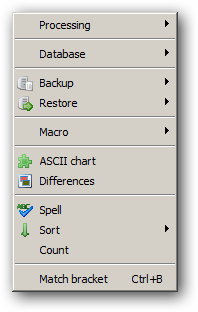
\includegraphics[scale=0.50]{./res/menu_tools.png}\\

\begin{scriptsize}\begin{tabularx}{\textwidth}{>{\hsize=0.2\hsize}X>{\hsize=0.8\hsize}X}\\
    \hline
    \textbf{Option} & \textbf{Description} \\
    \hline
    Processing & \textit{\htmladdnormallink{See options ...}{\#menu\_tools\_processing}} \\
    Database & \textit{\htmladdnormallink{See options ...}{\#menu\_tools\_database}} \\
    Backup & \textit{\htmladdnormallink{See options ...}{\#menu\_tools\_backup}} \\
    Restore & \textit{\htmladdnormallink{See options ...}{\#menu\_tools\_restore}} \\
    Macro & \textit{\htmladdnormallink{See options ...}{\#menu\_tools\_macro}} \\
    ASCII chart & Allows you to insert an active char to the active document \\
    Differences & Opens the nice TextDiff command by Angus Johnson integrated within Tinn-R \\
    Spell & Starts the speller (\htmladdnormallink{see instructions ...}{\#working\_tools\_spell}) \\
    Sort & \textit{\htmladdnormallink{See options ...}{\#menu\_tools\_sort}} \\
    Count & Shows the result of the count action (words, characters + spaces, character - spaces and spaces) for files or a text selection \\
    Match bracket & Search for matching bracket. See details below \\
    \hline
  \end{tabularx}\end{scriptsize}

\begin{description}
  \item[How to match:]
    The cursor must be placed immediately before any of the bracket characters.  When this option is called the cursor will move to the point immediately before the matching bracket.

  \item[Recognized brackets:]
    The bracket characters are (), [] and \{\}.
\end{description}


\hypertarget{menu_tools_processing}{}
\subsection{Processing}
\index{tools menu!processing}

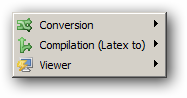
\includegraphics[scale=0.50]{./res/menu_tools_processing.png}\\

\begin{scriptsize}\begin{tabularx}{\textwidth}{>{\hsize=0.3\hsize}X>{\hsize=0.7\hsize}X}\\
    \hline
    \textbf{Option} & \textbf{Description} \\
    \hline
    Conversion & \textit{\htmladdnormallink{See options ...}{\#menu\_tools\_processing\_conversion}} \\
    Compilation (LaTeX to) & \textit{\htmladdnormallink{See options ...}{\#menu\_tools\_processing\_conversion\_compilation}} \\
    Viewer & \textit{\htmladdnormallink{See options ...}{\#menu\_tools\_processing\_viewer}} \\
    \hline
  \end{tabularx}\end{scriptsize}


\hypertarget{menu_tools_processing_conversion}{}
\subsubsection{Conversion}\\
\index{tools menu!processing}

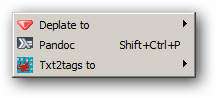
\includegraphics[scale=0.50]{./res/menu_tools_processing_conversion.png}\\

\begin{scriptsize}\begin{tabularx}{\textwidth}{>{\hsize=0.3\hsize}X>{\hsize=0.7\hsize}X}\\
    \hline
    \textbf{Option} & \textbf{Description} \\
    \hline
    Deplate to & \textit{\htmladdnormallink{See options ...}{\#menu\_tools\_processing\_conversion\_deplate}} \\
    Pandoc & \textit{\htmladdnormallink{See options ...}{\#menu\_tools\_processing\_conversion\_pandoc}} \\
    Txt2tags to & \textit{\htmladdnormallink{See options ...}{\#menu\_tools\_processing\_conversion\_txt2tags}} \\
    \hline
  \end{tabularx}\end{scriptsize}

\hypertarget{menu_tools_processing_conversion_deplate}{}
\subsubsection{Deplate to}\\
\index{tools menu!conversion deplate}

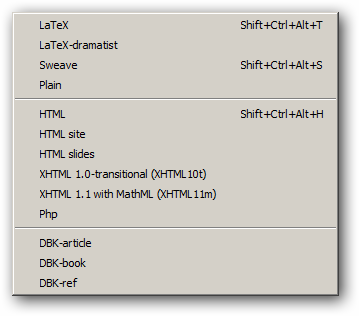
\includegraphics[scale=0.50]{./res/menu_tools_processing_conversion_deplate.png}\\

\begin{scriptsize}\begin{tabularx}{\textwidth}{>{\hsize=0.6\hsize}X>{\hsize=0.7\hsize}X}\\
    \hline
    \textbf{Option} & \textbf{Description} \\
    \hline
    LaTeX & Converts a Deplate file to LaTeX \\
    LaYeX-dramatist & Converts a Deplate file to LaTeX-dramatist \\
    Sweave & Converts a Deplate file to Sweave \\
    Plain & Converts a Deplate file to Plain \\
    HTML & Converts a Deplate file to HTML \\
    HTML site & Converts a Deplate file to HTML site \\
    HTML slides & Converts a Deplate file to HTML slides \\
    XHTML 1.0 transitional (xhtml10t) & Converts a Deplate file to XHTML 1.0 transitional \\
    XHTML 1.1 with MathML (xhtml11m) & Converts a Deplate file to XHTML 1.1 with MathML \\
    PHP & Converts a Deplate file to PHP \\
    Dbk-article & Converts a Deplate file to Dbk-article \\
    Dbk-book & Converts a Deplate file to Dbk-book \\
    Dbk-ref & Converts a Deplate file to Dbk-ref \\
    \hline
  \end{tabularx}\end{scriptsize}

Tip: \htmladdnormallink{see details ...}{http://deplate.sourceforge.net/Output.html}


\newpage
\hypertarget{menu_tools_processing_conversion_pandoc}{}
\paragraph{}\textbf{Pandoc}\\

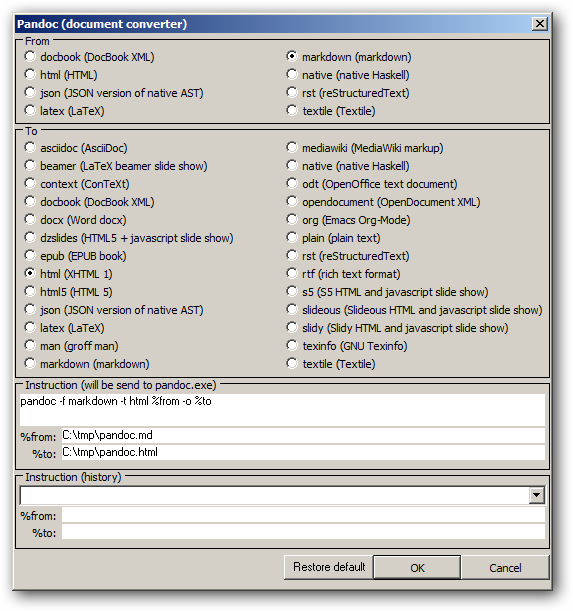
\includegraphics[scale=.50]{./res/pandoc.png}

Tip: \htmladdnormallink{see details ...}{http://johnmacfarlane.net/pandoc/index.html}


\hypertarget{menu_tools_processing_conversion_txt2tags}{}
\subsubsection{Txt2tags to}\\
\index{tools menu!processing Txt2tags}

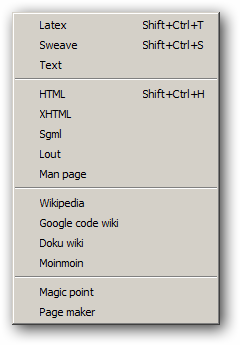
\includegraphics[scale=0.50]{./res/menu_tools_processing_conversion_txt2tags.png}\\

\begin{scriptsize}\begin{tabularx}{\textwidth}{>{\hsize=0.3\hsize}X>{\hsize=0.7\hsize}X}\\
    \hline
    \textbf{Option} & \textbf{Description} \\
    \hline
    LaTeX & Converts a Txt2tags file into LaTeX \\
    Sweave & Converts a Txt2tags file into Sweave \\
    Txt & Converts a Txt2tags file into txt \\
    HTML & Converts a Txt2tags file into HTML \\
    XHTML & Converts a Txt2tags file into XHTML \\
    SGML & Converts a Txt2tags file into SGML \\
    Lout & Converts a Txt2tags file into Lout \\
    Man page & Converts a Txt2tags file into Man page \\
    Wikipedia & Converts a Txt2tags file into Wikipedia \\
    Google code wiki & Converts a Txt2tags file into Google code wiki \\
    Doku wiki & Converts a Txt2tags file into Doku wiki \\
    Moinmoin & Converts a Txt2tags file into Moinmoin \\
    Magic point & Converts a Txt2tags file into Magic point \\
    Page maker & Converts a Txt2tags file into Page maker \\
    \hline
  \end{tabularx}\end{scriptsize}

Tip: \htmladdnormallink{see details ...}{http://txt2tags.sourceforge.net/}


\hypertarget{menu_tools_processing_conversion_compilation}{}
\subsubsection{Compilation (latex to)}\\
\index{tools menu!compilation}

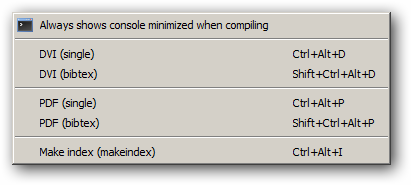
\includegraphics[scale=0.50]{./res/menu_tools_processing_compilation.png}\\

\begin{scriptsize}\begin{tabularx}{\textwidth}{>{\hsize=0.5\hsize}X>{\hsize=0.7\hsize}X}\\
    \hline
    \textbf{Option} & \textbf{Description} \\
    \hline
    Always shows console minimized when compiling & When this option is set the DOS console will be minimized when compiling \\
    DVI (single) & Compiles a LaTeX file to DVI in single way \\
    DVI (bibtex) & Compiles a LaTeX file to DVI in bibtex way (three compilation) \\
    Pdf (single) & Compiles a LaTeX file to PDF in single way \\
    Pdf (bibtex) & Compiles a LaTeX file to PDF in bibtex way (three compilation) \\
    \hline
  \end{tabularx}\end{scriptsize}


\hypertarget{menu_tools_processing_viewer}{}
\subsubsection{Viewer}\\
\index{tools menu!processing viewer}

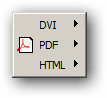
\includegraphics[scale=0.50]{./res/menu_tools_processing_viewer.png}\\

\begin{scriptsize}\begin{tabularx}{\textwidth}{>{\hsize=0.3\hsize}X>{\hsize=0.7\hsize}X}\\
    \hline
    \textbf{Option} & \textbf{Description} \\
    \hline
    DVI & \textit{\htmladdnormallink{See options ...}{\#menu\_tools\_processing\_viewer\_DVI}} \\
    PDF & \textit{\htmladdnormallink{See options ...}{\#menu\_tools\_processing\_viewer\_pdf}} \\
    HTML & \textit{\htmladdnormallink{See options ...}{\#menu\_tools\_processing\_viewer\_html}} \\
    \hline
  \end{tabularx}\end{scriptsize}


\hypertarget{menu_tools_processing_viewer_DVI}{}
\subsubsection{DVI}\\
\index{tools menu!processing viewer dvi}

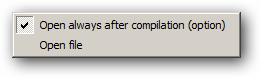
\includegraphics[scale=0.50]{./res/menu_tools_processing_viewer_dvi.png}\\

\begin{scriptsize}\begin{tabularx}{\textwidth}{>{\hsize=0.7\hsize}X>{\hsize=0.7\hsize}X}\\
    \hline
    \textbf{Option} & \textbf{Description} \\
    \hline
    Open always after compilation (option) & When this option is set the DVI file will be opened by the viewer after the compilation \\
    Open file & Shows the \textit{Windows Open dialog} to select a DVI file to be opened by the viewer \\
    \hline
  \end{tabularx}\end{scriptsize}


\hypertarget{menu_tools_processing_viewer_pdf}{}
\subsubsection{Pdf}\\
\index{tools menu!processing viewer pdf}

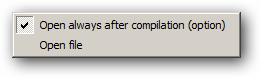
\includegraphics[scale=0.50]{./res/menu_tools_processing_viewer_pdf.png}\\

\begin{scriptsize}\begin{tabularx}{\textwidth}{>{\hsize=0.7\hsize}X>{\hsize=0.7\hsize}X}\\
    \hline
    \textbf{Option} & \textbf{Description} \\
    \hline
    Open always after compilation (option) & When this option is set the Pdf file will be opened by the viewer after the compilation \\
    Open file & Shows the \textit{Windows Open dialog} to select a DVI file to be opened by the viewer \\
    \hline
  \end{tabularx}\end{scriptsize}


\hypertarget{menu_tools_processing_viewer_html}{}
\subsubsection{Html}\\
\index{tools menu!processing viewer html}

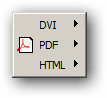
\includegraphics[scale=0.50]{./res/menu_tools_processing_viewer.png}\\

\begin{scriptsize}\begin{tabularx}{\textwidth}{>{\hsize=0.7\hsize}X>{\hsize=0.7\hsize}X}\\
    \hline
    \textbf{Option} & \textbf{Description} \\
    \hline
    Open always after conversion (option) & When this option is set the Html file will be opened by the viewer after the compilation \\
    Open current file & Opens the current DVI file with the viewer \\
    Open file & Shows the \textit{Windows Open dialog} to select a DVI file to be opened by the viewer \\
    \hline
  \end{tabularx}\end{scriptsize}


\hypertarget{menu_tools_database}{}
\subsection{Database}
\index{tools!database}

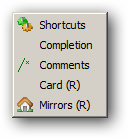
\includegraphics[scale=0.50]{./res/menu_tools_database.png}\\

\begin{scriptsize}\begin{tabularx}{\textwidth}{>{\hsize=0.3\hsize}X>{\hsize=0.7\hsize}X}\\
    \hline
    \textbf{Option} & \textbf{Description} \\
    \hline
    Shortcuts & Shows Shortcuts database (XML based) dialog \\
    Completion & Shows Completion database (XML based) dialog \\
    Comments & Shows Comments database (XML based) dialog \\
    Card (R) & Shows R card database (XML based) dialog \\
    Mirrors (R) & Shows R mirrors database (XML based) dialog \\
    \hline
  \end{tabularx}\end{scriptsize}


\hypertarget{menu_tools_backup}{}
\subsection{Backup}
\index{tools!backup}

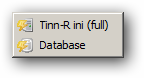
\includegraphics[scale=0.50]{./res/menu_tools_backup.png}\\

\begin{scriptsize}\begin{tabularx}{\textwidth}{>{\hsize=0.3\hsize}X>{\hsize=0.7\hsize}X}\\
    \hline
    \textbf{Option} & \textbf{Description} \\
    \hline
    System configuration & Backups Tinn-R configuration (ini files) \\
    Database & Backups database (Cachexml, Comments.xml, Completions.xml, Rcard.xml, Rmirrors.xml and Shortcuts.xml) \\
    \hline
  \end{tabularx}\end{scriptsize}


\hypertarget{menu_tools_restore}{}
\subsection{Restore}
\index{tools!restore}

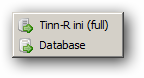
\includegraphics[scale=0.50]{./res/menu_tools_restore.png}\\

\begin{scriptsize}\begin{tabularx}{\textwidth}{>{\hsize=0.3\hsize}X>{\hsize=0.7\hsize}X}\\
    \hline
    \textbf{Option} & \textbf{Description} \\
    \hline
    System configuration & Restores a prior Tinn-R backup (ini files) \\
    Database & Restores a prior database backup (Cachexml, Comments.xml, Completions.xml, Rcard.xml, Rmirrors.xml and Shortcuts.xml) \\
    \hline
  \end{tabularx}\end{scriptsize}


\hypertarget{menu_tools_macro}{}
\subsection{Macro}
\index{tools!macro}

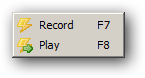
\includegraphics[scale=0.50]{./res/menu_tools_macro.png}\\

\begin{scriptsize}\begin{tabularx}{\textwidth}{>{\hsize=0.3\hsize}X>{\hsize=0.7\hsize}X}\\
    \hline
    \textbf{Option} & \textbf{Description} \\
    \hline
    Record & Toggles macro recording on and off. Note that when recording a macro the button changes \\
    Play & Plays a previous recorded macro \\
    \hline
  \end{tabularx}\end{scriptsize}

\textbf{It is not possible to save/edit macros, they are temporary}


\hypertarget{menu_tools_sort}{}
\subsection{Sort}
\index{tools!sort}

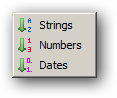
\includegraphics[scale=0.50]{./res/menu_tools_sort.png}\\

\begin{scriptsize}\begin{tabularx}{\textwidth}{>{\hsize=0.3\hsize}X>{\hsize=0.7\hsize}X}\\
    \hline
    \textbf{Option} & \textbf{Description} \\
    \hline
    Strings & Sorts strings \\
    Numbers & Sorts numbers \\
    Dates & Sorts dates \\
    \hline
  \end{tabularx}\end{scriptsize}

\textbf{Sort works on the entire document unless some text is selected}
